\part{Mechanik}
\chapter{Bewegungen} %gleichförmige bewegung, gleichmässig beschleunigte bewegung (freier fall), 2d bewegungen (würfe (vertikaler wurf, horizontaler wurf), 
\section{Die gleichförmige Bewegung}

Unter dem Begriff \textbf{Geschwindigkeit} $v$ versteht man die von einem Körper zurückgelegte Wegstrecke $\Delta s$ pro Zeiteinheit $\Delta t$. Also:

\[ v = \frac{\Delta s}{\Delta t} \]

Die Einheit von $v$ wird in den Grundeinheiten angegeben:

\[ \left[ v \right] = \si{\metre \per \second} \]


\begin{regel}Umrechnung von \si{\kilo \metre \per \hour} zu \si{\metre \per \second} und umgekehrt
\vspace{3cm}
\end{regel}
Die Geschwindigkeit ist bei einer gleichförmigen Bewegung konstant. 
\begin{itemize}
    \item \textbf{Momentangeschwindigkeit $v_{m}$}: Die Momentangeschwindigkeit ist die Geschwindigkeit eines Körpers zu einem bestimmten Zeitpunkt. Wenn sich der Körper mit konstanter Geschwindigkeit fortbewegt, so ist die Momentangeschwindigkeit immer gleich gross.
	\item \textbf{Durchschnittsgeschwindigkeit $\bar{v}$}: Die Durchschnittsgeschwindigkeit wird über den ganzen Bewegungsablauf berechnet und entspricht bei einer Bewegung mit konstanter Geschwindigkeit stets der Momentangeschwindigkeit.
\end{itemize}

\subsection{Diagramme}

Um einen Bewegungsablauf eines Körpers besser erfassen zu können, wird seine Bewegung in einem Diagramm beschrieben. Wir unterscheiden:
\begin{itemize}
	\item \textbf{Zeit-Ort-Diagramm}: Auf der $x$-Achse wird die Zeit $t$, auf der $y$-Achse der Weg (Strecke) $s$ dargestellt. Bewegungen mit konstanter Geschwindigkeit entsprechen in diesem Diagramm geraden Linien.
	\item \textbf{Zeit-Geschwindigkeits-Diagramm}: Auf der $x$-Achse wird die Zeit $t$, auf der $y$-Achse die Momentangeschwindigkeit (Strecke) $\bar{v}$ (oder auch $v(t)$) dargestellt. Bewegungen mit konstanter Geschwindigkeit entsprechen in diesem Diagramm horizontalen Linien.
\end{itemize}
Wir betrachten zuerst das \textbf{Zeit-Ort-Diagramm}:

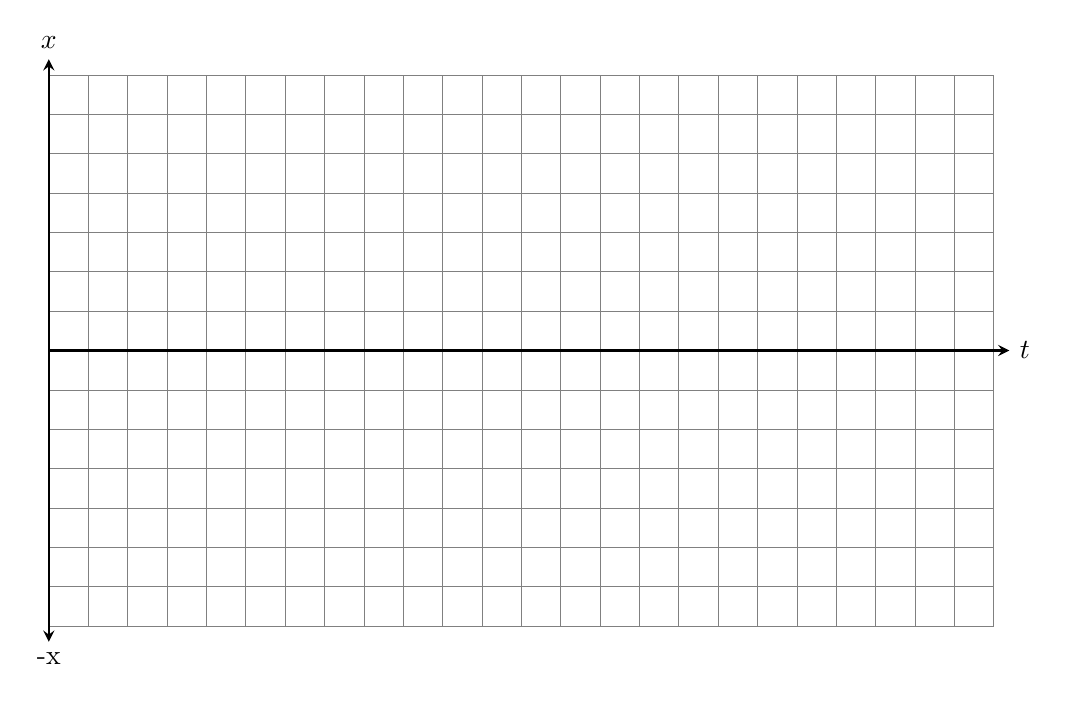
\begin{tikzpicture}
        \draw[step=0.5cm,gray,very thin] (0,0) grid (12,7);
        \draw[thick,-stealth] (0,3.5) -- (12.2,3.5) node[right] {$t$};
        \draw[thick, stealth-stealth] (0,-0.2) node[below] {-x} -- (0,7.2) node[above] {$x$};
\end{tikzpicture}

Als nächstes betrachten wir das \textbf{Zeit-Geschwindigkeits-Diagramm}:

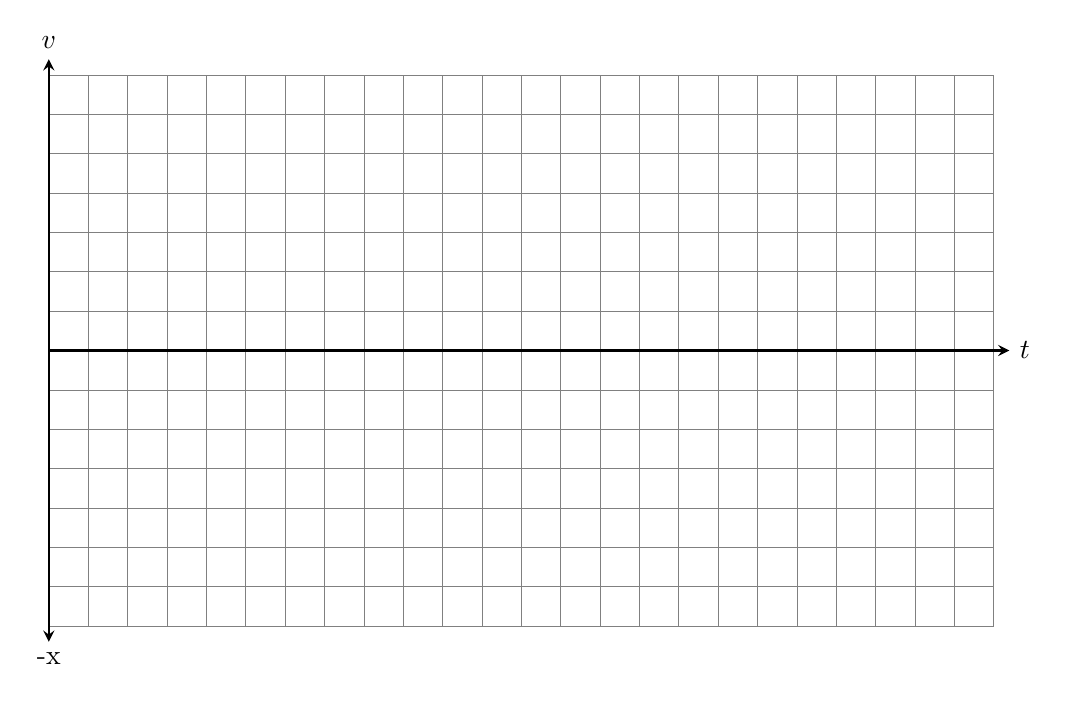
\begin{tikzpicture}
        \draw[step=0.5cm,gray,very thin] (0,0) grid (12,7);
        \draw[thick,-stealth] (0,3.5) -- (12.2,3.5) node[right] {$t$};
        \draw[thick, stealth-stealth] (0,-0.2) node[below] {-x} -- (0,7.2) node[above] {$v$};
\end{tikzpicture}

Ein Bewegungsablauf lässt sich immer in beiden Diagrammen darstellen. Eine gleichförmige Bewegung lässt sich an den folgenden Merkmalen in den Diagrammen erkennen:
\begin{itemize}
\item im Zeit-Weg-Diagramm ist der Graph stets eine gerade Linie
\item im Zeit-Geschwindigkeit-Diagramm ist der Graph stets eine horizontale Linie
\end{itemize}
\newpage

\section{Die beschleunigte Bewegung}
\begin{marginfigure}
    \includegraphics[width=0.9\textwidth]{Bilder/beschleunigung.jpg}
\end{marginfigure}
Unter dem Begriff \textbf{Beschleunigung} $a$ versteht man die Änderung des Bewegungszustandes. Ändert mindestens eine der folgenden Grössen, dann liegt eine beschleunigte Bewegung vor:
\begin{itemize}
\item der Betrag der Geschwindigkeit $v$
\item die Richtung der Geschwindigkeit $\vec{v}$
\end{itemize}
Wir konzentrieren uns zunächst auf die Änderung des Geschwindigkeitsbetrages. Somit gilt:
\begin{definition}
\[ a = \frac{\Delta v}{\Delta t} = \frac{\text{Geschwindigkeitsänderung}}{\text{Zeitdauer}}\]
\end{definition}
Die Definitionsgleichung gilt nur für:
\begin{itemize}
	\item gleichmässig beschleunigte Bewegungen ($a=\text{konstant}$)
	\item gilt annähernd für die Augenblicksbeschleunigung
\end{itemize}
Bei ungleichmässig beschleunigten Bewegungen muss mit einer mittleren Beschleunigung (Durchschnittsbeschleunigung) $\overline{a}$ gerechnet werden!
Die Einheit von $a$ wird in den Grundeinheiten angegeben:
\[ [a] = \si{\metre \per \second \squared} \]
Die Beschleunigung gibt also an, um wie viele Meter pro Sekunde sich eine Geschwindigkeit pro Sekunde ändert.
Ändert sich also die Geschwindigkeit eines bewegten Körpers, etwa eines Autos, wenn der Fahrer ``Gas gibt'' oder abbremst, so führt er eine beschleunigte Bewegung aus, eine Beschleunigung liegt aber auch vor, wenn sich nur die Richtung der Geschwindigkeit ändert, also wenn das Auto eine Kurve fährt. Beispiele:
\begin{example}
\begin{itemize}
	\item Anfahren eines Autos auf gerader Strecke $\Rightarrow$ 
	\item Auto fährt durch Kurve $\Rightarrow$ 
\end{itemize}
\end{example}
Beschleunigung ist eine \textbf{gerichtete Grösse}, besitzt also Betrag und Richtung, wie auch die Geschwindigkeit. Die Beschleunigung lässt sich also auch mit einem Pfeil\marginnote{Die Länge des Pfeils enstspricht dabei dem Betrag der Beschleunigung, der Pfeil wird \textbf{Vektor} genannt} darstellen. Ist die Beschleunigung positiv, so wird das Objekt schneller, ist die Beschleunigung hingegen negativ, so sprechen wir vom Abbremsen.

\begin{example}
Ein Auto, das aus dem Stillstand in \SI{10}{\second} die Geschwindigkeit von \SI{100}{\kilo \metre \per \hour} erreicht, beschleunigt mit
\[ a= \frac{\Delta v}{\Delta t} = \frac{\SI{27.8}{\metre \per \second} - \SI{0}{\metre \per \second}}{\SI{10}{\second}} = \SI{2.78}{\metre \per \second \squared} \]
\end{example}
\begin{marginfigure}
    \includegraphics[width=0.7\textwidth]{Bilder/zikade.jpg}
    \caption{Aufnahme des Absprungs der Wiesenschaumzikade mit einer Kamera die 2000 Bilder pro Sekunde macht.}
\end{marginfigure}
\begin{example}
Die Wiesenschaumzikade (Philaenus spumarius) kann mit der unglaublichen Beschleunigung von \SI{4}{\kilo \metre \per \second \squared} abspringen. Diese Beschleunigung wirkt aber nur über ca. \SI{0.8}{\milli \second}. Welche Geschwindigkeit erreicht die Zikade?
\[ a= \frac{\Delta v}{\Delta t} \]
Auflösen nach $\Delta v$:
\[ \Delta v = a \cdot \Delta t =  \SI{4E3}{ \metre \per \second \squared} \cdot \SI{8E-4}{\second} = \SI{3.2}{\metre \per \second}\]

\end{example} \newpage
\subsection{Diagramme}
Die beschleunigte Bewegung lässt sich auch in den bereits bekannten Diagrammen darstellen: 
Wir betrachten zuerst die gleichmässig beschleunigte Bewegung im \textbf{Zeit-Ort-Diagramm}:

\begin{figure}
\begin{tikzpicture}
        %\draw[step=0.5cm,gray,very thin] (0,0) grid (12,7);
        \begin{axis}[
        width=0.95\textwidth,
      xmin=0, xmax=7.5,ymin=0,ymax=13,domain=0:7,
      axis lines =center, xlabel=$t$ in s, ylabel=$x$ in m,
      every axis y label/.style={at=(current axis.above origin),anchor=south},
      every axis x label/.style={at=(current axis.right of origin),anchor=west},
      axis on top,
      grid=major,
    ] 
    
    \addplot [penColor,very thick,smooth] {0.5*0.5*x^2};
  \end{axis}
\end{tikzpicture}
\caption{$t$-$x$-Diagramm einer gleichmässig beschleunigten Bewegung mit $a=\SI{0.5}{\metre \per \second \squared}$}, Startpunkt bei $x=\SI{0}{\metre}$
\end{figure}

Die Steigung der Kurve nimmt ständig zu: Die Steigung in diesem Diagramm entspricht ja bekanntlich der Geschwindigkeit, diese nimmt bei einer positiven Beschleunigung zu. Ist die Beschleunigung $a<0$, so nimmt die Geschwindigkeit laufend ab. \newpage
Betrachten wir nun die gleiche Bewegung im Zeit-Geschwindigkeits-Diagramm:

\begin{figure}
\begin{tikzpicture}
        %\draw[step=0.5cm,gray,very thin] (0,0) grid (12,7);
        \begin{axis}[
        width=0.95\textwidth,
      xmin=0, xmax=7.5,ymin=0,ymax=4,domain=0:7,
      axis lines =center, xlabel=$t$ in s, ylabel=$v$ in \si{\metre \per \second},
      every axis y label/.style={at=(current axis.above origin),anchor=south},
      every axis x label/.style={at=(current axis.right of origin),anchor=west},
      axis on top,
      grid=major,
    ] 
    \addplot [draw=none,fill=fillp,domain=(0:7)] {0.5*x} \closedcycle;
    \addplot [penColor,very thick,smooth] {0.5*x};
  \end{axis}
\end{tikzpicture}
\caption{$t$-$v$-Diagramm einer gleichmässig beschleunigten Bewegung mit $a=\SI{0.5}{\metre \per \second \squared}$. $v_{0} = \SI{0}{\metre \per \second}$}
\end{figure}

Die Steigung dieser Kurve ist konstant: Die Steigung in diesem Diagramm entspricht der Beschleunigung, diese beträgt während des gesamten Bewegungsablaufs konstant $a=\SI{0.5}{\metre \per \second \squared}$. Die Fläche unter der Kurve (eingefärbt) entspricht der zurückgelegten Strecke. Die Fläche (zurückgelegte Strecke $\Delta s$) wird berechnet mit:
\[ \Delta s = \frac{\Delta v \cdot \Delta t}{2} = \frac{1}{2} \Delta v \Delta t = \frac{1}{2} a  t^{2} \]
\newpage
Betrachten wir nun noch ein neues Diagramm, das Zeit-Beschleunigungs-Diagramm:

\begin{figure}
\begin{tikzpicture}
        %\draw[step=0.5cm,gray,very thin] (0,0) grid (12,7);
        \begin{axis}[
        width=0.95\textwidth,
      xmin=0, xmax=7.5,ymin=0,ymax=1,domain=0:7,
      axis lines =center, xlabel=$t$ in s, ylabel=$a$ in \si{\metre \per \second \squared},
      every axis y label/.style={at=(current axis.above origin),anchor=south},
      every axis x label/.style={at=(current axis.right of origin),anchor=west},
      axis on top,
      grid=major,
    ] 
    \addplot [draw=none,fill=fillp,domain=(0:7)] {0.5} \closedcycle;
    \addplot [penColor,very thick,smooth] {0.5};
  \end{axis}
\end{tikzpicture}
\caption{$t$-$a$-Diagramm einer gleichmässig beschleunigten Bewegung mit $a=\SI{0.5}{\metre \per \second \squared}$}
\end{figure}

Die Steigung dieser Kurve ist Null. Die Steigung in diesem Diagramm entspricht der Änderung der Beschleunigung, diese ist jedoch konstant, ändert sich also nicht. Die eingefärbte Fläche entspricht der Änderung der Geschwindigkeit:
\[ \Delta v = a \Delta t \]

\subsection{Messung der Beschleunigung} %moutionmountain 1 (S.82)
In einem gewöhnlichen Auto oder auf einem Motorrad können wir die Beschleunigung \textit{spüren} (diese Beschleunigungen liegen unter der Stärke von \SI{1}{g}\marginnote{eine Beschleunigung von \SI{1}{g} entspricht \SI{9.81}{\metre \per \second \squared}} und sind somit ungefährlich). Wir spüren Beschleunigung, da in uns ein Teil des Körpers gegen einen anderen Teil bewegt wird; Beschleunigung deformiert uns. Ein solcher bewegter Teil kann zum Beispiel ein kleiner Bestandteil des Innern des Ohres, der Magen im Bauch oder auch einfach die Glieder am Rumpf sein. Alle Beschleunigungs-Sensoren, auch diejenigen in der Tabelle unten oder den Abbildungen~\ref{fig:mems} bis~\ref{fig:sacculus} , egal ob biologisch oder technisch, funktionieren auf diese Art und Weise. 
\begin{marginfigure}
    \includegraphics[width=0.9\textwidth]{Bilder/mems.jpg}
    \caption{Ein mikro-elektro-mechanischer Beschleunigungssensor (MEMS) aus einem Smartphone}
\label{fig:mems}
\end{marginfigure}

\begin{marginfigure}
    \includegraphics[width=0.7\textwidth]{Bilder/piezo.jpg}
    \caption{Ein piezoelektrischer Beschleunigungssensor mit 3 Achsen}
\label{fig:piezo}
\end{marginfigure}

\begin{table}
\begin{longtable}{@{} m{5cm} m{5cm} m{2cm} @{}}
\toprule
Messung & Sensor & Messbereich \\
\midrule
Richtung der Gravitation in Pflanzen (Wurzeln, Stamm, Zweige, Blätter) & Amyloplasten in speziellen Zellen (Statocytenzellen) & 0 bis \SI{10}{\metre \per \second \squared} \\
Richtung und Stärke der Gravitation in Säugetieren & Die Memberanen in den Bogengängen und Sacculus und Utriculus (Makulaorgane) im Innenohr & 0 bis \SI{20}{\metre \per \second \squared} \\
Richtung und Betrag der Beschleunigung in Schrittzählern (Pedometer) für Wanderer & Piezoelektrische Sensoren & 0 bis \SI{20}{\metre \per \second \squared} \\
Richtung und Betrag der Beschleunigung in Smartphones & Mikro-elektro-mechanischer Sensor (MEMS) & 0 bis \SI{200}{\metre \per \second \squared} \\
Richtung und Betrag der Beschleunigung bei Autounfällen & Airbag Sensor, (Mikro-Elektro-mechanischer Sensor) & 0 bis \SI{2000}{\metre \per \second \squared} \\
\bottomrule
\end{longtable}
\end{table}
In Smartphones werden heute Beschleunigungssensoren verbaut, um damit die räumliche Orientierung des Geräts zu bestimmen. Das ermöglicht zum Beispiel dann den Bildschirminhalt entsprechend zu drehen. Diese Beschleunigungssensoren lassen sich durch entsprechende Apps auslesen, damit kann ein Smartphone als Beschleunigungs-Messgerät verwedent werden. Probieren Sie das einmal aus! \newpage
\begin{marginfigure}
    \includegraphics[width=1\textwidth]{Bilder/innenohr.jpg}
    \caption{Die Beschleunigungssensoren des Menschen liegen im Innenohr}
\label{fig:innenohr}
\end{marginfigure}

\begin{marginfigure}
    \includegraphics[width=1\textwidth]{Bilder/sacculus.jpg}
    \caption{Die Lage der Maculaorgane Sacculus und Ultriculus im Innenohr}
\label{fig:sacculus}
\end{marginfigure}

In der untenstehenden Tabelle sind einige Beschleunigungswerte angegeben:
\begin{table}
\begin{longtable}{@{} m{9.5cm} m{2.5cm}  @{}}
\toprule
Beobachtung & Beschleunigung  \\
\midrule
%Rückbeschleunigung der Galaxie M82 durch den ausgestossenen Jet & \SI{10}{\femto \metre \per \second \squared} \\
Beschleunigung eines jungen Sternes durch ausgestossenes Material (Jet) & \SI{10}{\pico \metre \per \second \squared} \\
%Beschleunigung der Sonne im Orbit um die Milchstrasse & \SI{0.2}{\nano \metre \per \second \squared} \\
Beschleunigung am Äquator durch die Erdrotation & \SI{33}{\nano \metre \per \second \squared} \\
Beschleunigung der Elektronen durch den Wechselstrom in gewöhnlichen Stromleitungen & \SI{50}{\milli \metre \per \second \squared} \\
Beschleunigung einer schnellen U-Bahn & \SI{1.3}{ \metre \per \second \squared} \\
Fallbeschleunigung auf dem Mond & \SI{1.6}{ \metre \per \second \squared} \\
Minimale gesetzlich vorgeschriebene Bremsbeschleunigung auf trockenem Asphalt für ein Auto & \SI{5.5}{ \metre \per \second \squared} \\
Durchschnittliche Fallbeschleunigung auf der Erde & \SI{9.81}{ \metre \per \second \squared} \\
Maximale Beschleunigung eines Autos oder Motorrades mit Verbrennungsmotor & \SI{15}{ \metre \per \second \squared} \\
Beschleunigung eines Gepards & \SI{32}{ \metre \per \second \squared} \\
Rakete beim Start & bis \SI{90}{ \metre \per \second \squared} \\
Beschleunigung einer Stubenfliege & ca. \SI{100}{ \metre \per \second \squared} \\
Beschleunigung eines geworfenen Steins & ca. \SI{120}{ \metre \per \second \squared} \\
Beschleunigung eines Airbags im Auto & \SI{360}{ \metre \per \second \squared} \\
Beschleunigung einer Patrone im Gewehr & \SI{2}{ \mega \metre \per \second \squared} \\
Beschleunigung von Protonen in grossen Teilchenbeschleunigern & \SI{90}{\tera \metre \per \second \squared} \\
Beschleunigung von Protonen im Atomkern & \SI{E31}{\metre \per \second \squared} \\
\bottomrule
\end{longtable}
\end{table}

\subsection{Beispiele}
\begin{example}
Ein Radfahrer beschleunigt sein Rad aus dem Stillstand mit $a=\SI{2}{\metre \per \second \squared}$. Berechnen Sie die Geschwindigkeit $v_{1}$ nach $t_{1} = \SI{2}{\second}$, und $v_{2}$ nach $t_{2}=\SI{7}{\second}$. Wie gross ist die mittlere Geschwindigkeit im Intervall $[t_{1},t_{2}]$?
\end{example}
\begin{solution}
Momentangeschwindigkeiten: 
\[v_{1}=a \cdot \Delta t = a \cdot t_{1} = \SI{4}{\metre \per \second} \] und 
\[ v_{2} = a \cdot \Delta t = a \cdot t_{2} = \SI{14}{\metre \per \second} \] 
Mittlere Geschwindigkeit (Durchschnittsgeschwindigkeit):
\[ \bar{v} = \frac{\Delta s}{\Delta t} = \frac{s_{2}-s_{1}}{t_{2}-t_{1}}\]
mit
\[ s_{2}-s_{1} = \frac{1}{2} \cdot a \cdot t_{2}^{2}-\frac{1}{2}\cdot a \cdot t_{1}^{2}= \SI{49}{m} - \SI{4}{m} = \SI{45}{\metre}\]
\[ \bar{v} = \frac{\SI{45}{\metre}}{\SI{5}{\second}} = \SI{9}{\metre \per \second} \]
Variante: Nur für Bewegungen mit konstanter Beschleunigung gilt:
\[ \bar{v} = \frac{v_{1} + v_{2}}{2} = \frac{\SI{4}{\metre \per \second} + \SI{14}{\metre \per \second}}{2} = \SI{9}{\metre \per \second} \]
Dieser Zusammenhang lässt sich im $t-v$-Diagramm zeigen.
\end{solution}

\begin{example}
Ein Automobilist fährt mit einer Geschwindigkeit $v_{0} = \SI{30}{\metre \per \second}$. Auf der Fahrbahn taucht ein Hindernis auf. Nach einer Reaktionszeit von \SI{1}{\second} bremst er mit $a=\SI{-3.0}{\metre \per \second \squared}$ ab und bleibt dann unmittelbar vor dem Hindernis stehen.
\begin{enumerate}
\item Welchen Weg $s_{R}$ legt das Auto während der Reaktionszeit des Fahrers zurück?
\item Wie gross ist der Bremsweg $s_{B}$ des Fahrzeugs?
\item In welchem Abstand $\Delta s'$ vom Hindernis kommt das Auto zum Stehen, wenn die Reaktionszeit des Fahrers nur $t_{R} = \SI{0.5}{\second}$ beträgt?
\item Mit welcher Geschwindigkeit $v''$ fährt er in das Hindernis hinein, wenn seine Reaktionszeit wegen Unaufmerksamkeit $t''=\SI{1.5}{\second}$ beträgt?
\end{enumerate}
\end{example}

\begin{solution}
Wir skizzieren dazu ein $t-v$-Diagramm (unten) und lösen grafisch:
\begin{enumerate}
\item $s_{R} = \SI{30}{m}$
\item $s_{B} = \SI{150}{m}$, total \SI{180}{m}
\item Es ändert sich nur die Reaktionszeit, und damit wird der Reaktionsweg halbiert. $\Delta s'=\SI{15}{m}$.
\item Nach \SI{45}{m} beginnt der Bremsvorgang, dann beträgt die Distanz zum Hindernis noch $s''=\SI{135}{m}$. Für die Geschwindigkeit erhält man:
\[ v=\sqrt{v_{0}^{2} + 2 \cdot a \cdot s''} = \SI{9.5}{\metre \per \second} = \SI{34.2}{\kilo \metre \per \second}\]
\end{enumerate}
\end{solution}
\begin{figure}
\begin{tikzpicture}
        %\draw[step=0.5cm,gray,very thin] (0,0) grid (12,7);
        \begin{axis}[
        width=0.95\textwidth,
      xmin=0, xmax=12,ymin=0,ymax=30,domain=0:12,
      axis lines =center, xlabel=$t$ in s, ylabel=$v$ in \si{\metre \per \second},
      every axis y label/.style={at=(current axis.above origin),anchor=south},
      every axis x label/.style={at=(current axis.right of origin),anchor=west},
      axis on top,
      grid=major,
    ] ;
  \end{axis}
\end{tikzpicture}
\end{figure}